% Options for packages loaded elsewhere
\PassOptionsToPackage{unicode}{hyperref}
\PassOptionsToPackage{hyphens}{url}
%
\documentclass[
  english,
  man]{apa6}
\usepackage{amsmath,amssymb}
\usepackage{lmodern}
\usepackage{ifxetex,ifluatex}
\ifnum 0\ifxetex 1\fi\ifluatex 1\fi=0 % if pdftex
  \usepackage[T1]{fontenc}
  \usepackage[utf8]{inputenc}
  \usepackage{textcomp} % provide euro and other symbols
\else % if luatex or xetex
  \usepackage{unicode-math}
  \defaultfontfeatures{Scale=MatchLowercase}
  \defaultfontfeatures[\rmfamily]{Ligatures=TeX,Scale=1}
\fi
% Use upquote if available, for straight quotes in verbatim environments
\IfFileExists{upquote.sty}{\usepackage{upquote}}{}
\IfFileExists{microtype.sty}{% use microtype if available
  \usepackage[]{microtype}
  \UseMicrotypeSet[protrusion]{basicmath} % disable protrusion for tt fonts
}{}
\makeatletter
\@ifundefined{KOMAClassName}{% if non-KOMA class
  \IfFileExists{parskip.sty}{%
    \usepackage{parskip}
  }{% else
    \setlength{\parindent}{0pt}
    \setlength{\parskip}{6pt plus 2pt minus 1pt}}
}{% if KOMA class
  \KOMAoptions{parskip=half}}
\makeatother
\usepackage{xcolor}
\IfFileExists{xurl.sty}{\usepackage{xurl}}{} % add URL line breaks if available
\IfFileExists{bookmark.sty}{\usepackage{bookmark}}{\usepackage{hyperref}}
\hypersetup{
  pdftitle={Effectiveness of distance Based suicide Intervention programs, a multi-level meta-analysis and systematic review.},
  pdfauthor={Jim Schmeckenbecher1, Katrin Rattner2, Robert J. Cramer3, Paul L. Plener4, Anna Baran5, \& Nestor D. Kapusta1},
  pdflang={en-EN},
  pdfkeywords={suicide, suicide prevention, meta-analysis, distance based intervention, remote intervention, e-based intervention},
  hidelinks,
  pdfcreator={LaTeX via pandoc}}
\urlstyle{same} % disable monospaced font for URLs
\usepackage{longtable,booktabs,array}
\usepackage{calc} % for calculating minipage widths
% Correct order of tables after \paragraph or \subparagraph
\usepackage{etoolbox}
\makeatletter
\patchcmd\longtable{\par}{\if@noskipsec\mbox{}\fi\par}{}{}
\makeatother
% Allow footnotes in longtable head/foot
\IfFileExists{footnotehyper.sty}{\usepackage{footnotehyper}}{\usepackage{footnote}}
\makesavenoteenv{longtable}
\usepackage{graphicx}
\makeatletter
\def\maxwidth{\ifdim\Gin@nat@width>\linewidth\linewidth\else\Gin@nat@width\fi}
\def\maxheight{\ifdim\Gin@nat@height>\textheight\textheight\else\Gin@nat@height\fi}
\makeatother
% Scale images if necessary, so that they will not overflow the page
% margins by default, and it is still possible to overwrite the defaults
% using explicit options in \includegraphics[width, height, ...]{}
\setkeys{Gin}{width=\maxwidth,height=\maxheight,keepaspectratio}
% Set default figure placement to htbp
\makeatletter
\def\fps@figure{htbp}
\makeatother
\setlength{\emergencystretch}{3em} % prevent overfull lines
\providecommand{\tightlist}{%
  \setlength{\itemsep}{0pt}\setlength{\parskip}{0pt}}
\setcounter{secnumdepth}{-\maxdimen} % remove section numbering
% Make \paragraph and \subparagraph free-standing
\ifx\paragraph\undefined\else
  \let\oldparagraph\paragraph
  \renewcommand{\paragraph}[1]{\oldparagraph{#1}\mbox{}}
\fi
\ifx\subparagraph\undefined\else
  \let\oldsubparagraph\subparagraph
  \renewcommand{\subparagraph}[1]{\oldsubparagraph{#1}\mbox{}}
\fi
% Manuscript styling
\usepackage{upgreek}
\captionsetup{font=singlespacing,justification=justified}

% Table formatting
\usepackage{longtable}
\usepackage{lscape}
% \usepackage[counterclockwise]{rotating}   % Landscape page setup for large tables
\usepackage{multirow}		% Table styling
\usepackage{tabularx}		% Control Column width
\usepackage[flushleft]{threeparttable}	% Allows for three part tables with a specified notes section
\usepackage{threeparttablex}            % Lets threeparttable work with longtable

% Create new environments so endfloat can handle them
% \newenvironment{ltable}
%   {\begin{landscape}\centering\begin{threeparttable}}
%   {\end{threeparttable}\end{landscape}}
\newenvironment{lltable}{\begin{landscape}\centering\begin{ThreePartTable}}{\end{ThreePartTable}\end{landscape}}

% Enables adjusting longtable caption width to table width
% Solution found at http://golatex.de/longtable-mit-caption-so-breit-wie-die-tabelle-t15767.html
\makeatletter
\newcommand\LastLTentrywidth{1em}
\newlength\longtablewidth
\setlength{\longtablewidth}{1in}
\newcommand{\getlongtablewidth}{\begingroup \ifcsname LT@\roman{LT@tables}\endcsname \global\longtablewidth=0pt \renewcommand{\LT@entry}[2]{\global\advance\longtablewidth by ##2\relax\gdef\LastLTentrywidth{##2}}\@nameuse{LT@\roman{LT@tables}} \fi \endgroup}

% \setlength{\parindent}{0.5in}
% \setlength{\parskip}{0pt plus 0pt minus 0pt}

% \usepackage{etoolbox}
\makeatletter
\patchcmd{\HyOrg@maketitle}
  {\section{\normalfont\normalsize\abstractname}}
  {\section*{\normalfont\normalsize\abstractname}}
  {}{\typeout{Failed to patch abstract.}}
\patchcmd{\HyOrg@maketitle}
  {\section{\protect\normalfont{\@title}}}
  {\section*{\protect\normalfont{\@title}}}
  {}{\typeout{Failed to patch title.}}
\makeatother
\shorttitle{Distance Based Interventions}
\keywords{suicide, suicide prevention, meta-analysis, distance   based intervention, remote intervention, e-based intervention\newline\indent Word count: 3908}
\DeclareDelayedFloatFlavor{ThreePartTable}{table}
\DeclareDelayedFloatFlavor{lltable}{table}
\DeclareDelayedFloatFlavor*{longtable}{table}
\makeatletter
\renewcommand{\efloat@iwrite}[1]{\immediate\expandafter\protected@write\csname efloat@post#1\endcsname{}}
\makeatother
\usepackage{csquotes}
\ifxetex
  % Load polyglossia as late as possible: uses bidi with RTL langages (e.g. Hebrew, Arabic)
  \usepackage{polyglossia}
  \setmainlanguage[]{english}
\else
  \usepackage[main=english]{babel}
% get rid of language-specific shorthands (see #6817):
\let\LanguageShortHands\languageshorthands
\def\languageshorthands#1{}
\fi
\ifluatex
  \usepackage{selnolig}  % disable illegal ligatures
\fi
\newlength{\cslhangindent}
\setlength{\cslhangindent}{1.5em}
\newlength{\csllabelwidth}
\setlength{\csllabelwidth}{3em}
\newenvironment{CSLReferences}[2] % #1 hanging-ident, #2 entry spacing
 {% don't indent paragraphs
  \setlength{\parindent}{0pt}
  % turn on hanging indent if param 1 is 1
  \ifodd #1 \everypar{\setlength{\hangindent}{\cslhangindent}}\ignorespaces\fi
  % set entry spacing
  \ifnum #2 > 0
  \setlength{\parskip}{#2\baselineskip}
  \fi
 }%
 {}
\usepackage{calc}
\newcommand{\CSLBlock}[1]{#1\hfill\break}
\newcommand{\CSLLeftMargin}[1]{\parbox[t]{\csllabelwidth}{#1}}
\newcommand{\CSLRightInline}[1]{\parbox[t]{\linewidth - \csllabelwidth}{#1}\break}
\newcommand{\CSLIndent}[1]{\hspace{\cslhangindent}#1}

\title{Effectiveness of distance Based suicide Intervention programs, a multi-level meta-analysis and systematic review.}
\author{Jim Schmeckenbecher\textsuperscript{1}, Katrin Rattner\textsuperscript{2}, Robert J. Cramer\textsuperscript{3}, Paul L. Plener\textsuperscript{4}, Anna Baran\textsuperscript{5}, \& Nestor D. Kapusta\textsuperscript{1}}
\date{}


\authornote{

Correspondence concerning this article should be addressed to Nestor D. Kapusta, Medical University Vienna, Department of Psychoanalysis and Psychotherapy, Waehringer Guertel 18-20, 1090 Wien. E-mail: \href{mailto:nestor.kapusta@meduniwien.ac.at}{\nolinkurl{nestor.kapusta@meduniwien.ac.at}}

}

\affiliation{\vspace{0.5cm}\textsuperscript{1} Department of Psychoanalysis and Psychotherapy, Medical University Vienna, Austria\\\textsuperscript{2} Chiemgau - Clinic Marquartstein, Germany\\\textsuperscript{3} Department of Public Health Sciences, University of North Carolina at Charlotte, USA\\\textsuperscript{4} Department of Child and Adolescent Psychiatry, Medical University Vienna, Austria \& Department of Child and Adolescent Psychiatry and Psychotherapy, University of Ulm, Germany\\\textsuperscript{5} Department of Psychiatry, Blekinge Hospital, Karlshamn, Schweden}

\abstract{
Background: Distance Based Interventions (DBI) to reduce suicidal thoughts and behaviours are an increasingly relevant intervention type. They are more affordable, scalable and available than traditional face-to-face interventions, helping to narrow the gap between needed and provided care. Aim: Evaluating the overall effectiveness of DBI against suicidal thoughts and behaviours. Methods: We systematically searched Web of Science, Scopus and Pubmed for all DBI's primarily aimed at reducing suicidal thoughts and behaviours. Data was meta-analysed using a robust variance estimation corrected multilevel meta-analysis. Results: 40 studies emerged, reporting 110 outcomes. Effectiveness reducing suicidal thoughts was low (SMD = -0.17 CI95\%{[}-0.24; -0.11{]}), against suicidal behaviours DBI's were significantly less effective (SMD= -0.06 CI95\%{[}-0.09; -0.03{]}). Human involvement had no significant impact on effectiveness. Conclusion: DBI's maybe an effective tool in a stepped care approach, especially for reducing suicidal thoughts. Future research should focus on the development of mass distributable autonomous programs against suicidal ideation and plans.
}



\begin{document}
\maketitle

\hypertarget{introduction}{%
\section{Introduction}\label{introduction}}

Suicidal thoughts and behaviours are both a challenge for public health and for service providers, given that annually 138 million people experience suicide ideation, 20.7 million people attempt suicide (Borges et al., 2010) and around 700,000 people die by suicide (World Health Organization, 2021). Still only 17\% to 56\% of persons experiencing suicidal thoughts and behaviours receive treatment (Bruffaerts et al., 2011). Besides these undressed needs, low treatment rates are linked to two structural barriers such as: Treatment cost and availability (Bruffaerts et al., 2011).

Improving affordability and accessibility of treatment means to provide suicide-specific care in terms of tailored interventions according to the patient's stage of suicidal progression (e.g., pre-motivation, ideation only, plan/attempt; (\textbf{oconnor2011?})), rather than using a one fits all solution. It has been suggested to implement a stepped care approach: least restrictive care at early stages and to increase restrictions gradually with advancement of suicidal progression (Jobes, Gregorian, \& Colborn, 2018). In this sense, easily available and affordable treatment can lower treatment barriers and involve individuals otherwise hesitating to seek help at early suicidal stages (Bruffaerts et al., 2011). Early interventions at the stage of suicide ideation, have been suggested to lower human suffering and to prevent future suicides (Zuromski et al., 2019).

Distance Based Interventions (DBI) are least restrictive treatments, in terms of local availability, affordability and available service hours. Under-serviced areas can be supported by both tele-health and apps. While in the short term the development and evaluation of Apps and tele-health interventions are expensive, these are less expensive and less resource-intensive than individual psychotherapy, when a large amount of people are treated.

During the past two decades a number of randomized control trials examining DBI have been published. Starting at the turn of the millennium, with studies using phone-calls (Evans, Morgan, Hayward, \& Gunnell, 1999) and post-cards (Motto \& Bostrom, 2001), leading to crisis hotlines and e-mail follow-ups (Luxton, Smolenski, Reger, Relova, \& Skopp, 2020). Recently the field has expanded to online programs (Franklin et al., 2016; B. A. J. van Spijker, van Straten, \& Kerkhof, 2014) and since the Covid-19 outbreak increasingly to tele-health approaches (Fernandez et al., 2021). Several Meta-analyses have been published on subsets of DBI (Milner, Carter, Pirkis, Robinson, \& Spittal, 2015; Torok et al., 2020).

To give recommendations for future research and clinical practice, our meta-analysis differentiated between autonomous DBI (aDBI) (i.e.~apps, online programs) and human DBI (hDBI) (phone calls, postcards, tele-health), which allows to investigate, whether the scalability of hDBI can be utilized without risking effectiveness. To reach as many suicidal individuals as possible in early stages of progression, distance based programs need to be scalable and cost-effective. aDBI have superior scalability compared to hDBI (Batterham et al., 2015), as they are less expensive per intervention, less restricted by available service hours, more translatable, and immediately available.

In order to draw practical conclusions we asked three questions, implemented as moderation analyses: (a) Whether DBI are effective against suicide ideation and/or against suicidal behaviours, (b) How stable these interventions are over time and (c) Whether effectiveness of such programs was independent from the chosen control groups (TAU/Attention Placebo/waitlist).

\hypertarget{methods}{%
\subsection{Methods}\label{methods}}

The systematic search followed the Preferred Reporting Items for Systematic Reviews and Meta-Analyses guidelines (Page et al., 2021) and was Pre-Registered on Prospero under the pre-registration number: CRD42020218791.

\hypertarget{systematic-search}{%
\subsection{Systematic Search}\label{systematic-search}}

Search strings were defined using repeated searches combining MeSH terms relating to suicide prevention OR intervention, with the intervention types, (e.g.) Letter, App, Web-based, OR distance. The resulting search string was tested and refined using two related meta-analyses, one on hDBI (Milner, Carter, Pirkis, Robinson, \& Spittal, 2015) and one aDBI (Torok et al., 2020) (see Appendix for final strings).

Once search strings were established, the first one hundred search results of Web of Science were examined together by the authors J.S. and K.R., establishing a common degree of understanding. After which, both authors independently searched Web of Science, Scopus and Pubmed; Systematic searches were last updated in December 2021 . Cohen's kappa between both authors was 0.806.

\hypertarget{inclusion-and-exclusion-criteria}{%
\subsection{Inclusion and exclusion criteria}\label{inclusion-and-exclusion-criteria}}

All peer reviewed randomized control trial studies were included, which investigated any form of DBI with at least one primary outcome being self-harming thoughts and/or behaviours, such as suicidal ideation, suicidal planning, suicide attempts, and suicide. Face-to-face meetings were allowed, if these were not part of the intervention - i.e.~for informing, testing or screening purposes.

All suicidal thoughts and behaviour outcomes of applicable studies were coded, excluding combined outcome measures, such as the total score of
Suicidal Behaviours Questionnaire-Revised (SBQ-R) which sums lifetime thoughts and behaviours in a total score.

\hypertarget{data-extraction-and-coding}{%
\subsection{Data Extraction and Coding}\label{data-extraction-and-coding}}

Data was coded independently by two authors (J.S and K.R.). Where possible non-imputed results, were coded. The following variables were extracted: Author, Year, control group of study, country of study, sample type, sample size, intervention type, sex ratio, mean age, mean age(\emph{SD}), the outcome name (e.g.~suicidal ideation), intervention duration in weeks, the participant attrition rate, the follow-up time, standard mean difference (\emph{SMD)} and variance of \emph{SMD}. In addition, all outcomes were coded for the moderation analysis into subgroups (see Table 1).

\begin{longtable}[]{@{}
  >{\raggedright\arraybackslash}p{(\columnwidth - 2\tabcolsep) * \real{0.15}}
  >{\raggedright\arraybackslash}p{(\columnwidth - 2\tabcolsep) * \real{0.85}}@{}}
\caption{Outcome allocation to Moderator Analyses}\tabularnewline
\toprule
Moderator group & \textbf{Outcome Name} \\
\midrule
\endfirsthead
\toprule
Moderator group & \textbf{Outcome Name} \\
\midrule
\endhead
Acts & Suicide, suicide attempts, self harming behaviours. \\
Thoughts & Suicidal thoughts, suicidal ideation, suicide plans. \\
Human involved & Phone calls, cognitive behavioural treatment, personalized letters or personalized e-mails. \\
Autonomous & Applications, websites, non-individualized letters or non-individualized e-mails. \\
TAU & TAU, enhanced TAU, intensive case monitoring, \\
Attention Placebo & Attention placebo, control article, journalling, attention control, control program, body positivity images. \\
waitlist & no contact, reminder letter at the end, waitlist, no interventions \\
\bottomrule
\end{longtable}

The authors compared finalized coding sheets, discussed differences and re-coded affected studies until a unanimous result was achieved.

\hypertarget{risk-of-bias-and-publication-bias}{%
\subsection{Risk of bias and publication bias}\label{risk-of-bias-and-publication-bias}}

Risk of bias was assessed using the RoB-2 (Sterne et al., 2019) and Trim and Fill was used as the publication bias detection (Fernández-Castilla et al., 2021; Renkewitz \& Keiner, 2019).

\hypertarget{statistical-method}{%
\subsection{Statistical Method}\label{statistical-method}}

To incorporate all outcomes of interest we used a three level meta-analysis (Cheung, 2019; Van den Noortgate, López-López, Marín-Martínez, \& Sánchez-Meca, 2015), with Robust variance estimation (RVE) (Hedges, Tipton, \& Johnson, 2010; Moeyaert et al., 2017). RVE return valid confidence intervals in presence of dependent data (Park \& Beretvas, 2019). While the three level model allowed for outcome-level heterogeneity investigation (Van den Noortgate, López-López, Marín-Martínez, \& Sánchez-Meca, 2013), RVE return valid confidence intervals in presence of dependent data (Park \& Beretvas, 2019). Models were fitted with restricted maximum likelihood estimation (REML), RVE correction was based on Pustejovsky and Tipton (2016).

Calculations were done in R (R Core Team, 2020) using the package metafor for the three level model (Viechtbauer, 2010) and the package clubSandwich (Pustejovsky, 2021) for the RVE correction. All data needed for full reproducibility are publicly available on Github.\footnote{Link: \href{https://github.com/jim-schmeckenbecher/Distance-based-Interventions}{\textless https://github.com/jim-schmeckenbecher/Distance-based-Interventions\textgreater{}}.}

\hypertarget{sensitivity-analysis}{%
\subsection{Sensitivity Analysis}\label{sensitivity-analysis}}

Given that NSSI (American Psychiatric Association, 2013) and suicidal behaviours (Joiner, 2005) differ qualitatively, we employed two sensitivity analyses: (a) Including Non-Suicidal Self-Injury (NSSI) as an outcome, (b) Excluding suicide deaths as an outcome.

\hypertarget{deviation-from-pre-registered-report}{%
\subsection{Deviation from Pre-Registered Report}\label{deviation-from-pre-registered-report}}

Given most recent developments in meta-analytical research we adapted the procedure as follows: Firstly, instead of a more complex multi-level model, we employed a hybrid model of RVE correction and multilevel methodology (Pustejovsky \& Tipton, 2021), thereby improving efficiency and reducing risk of bias. Secondly, we followed the publication bias detection method recommended by Fernández-Castilla et al. (2021) instead of that by Renkewitz and Keiner (2019) although for this data set, both recommend the same method.

\hypertarget{results}{%
\section{Results}\label{results}}

\hypertarget{emerged-data}{%
\subsection{Emerged Data}\label{emerged-data}}

We identified 2,213 papers in the databases (see Flow Chart), in the end 35 independent RCT trials were included in the analysis. The difference between included studies in the flow chart and reported independent RCT trials is explained by follow-up studies that use the same sample as their parent study. As these study pairs have the same sample we treated them as a single RCT. Further, one study included three statistically independent RCTs (Franklin et al., 2016).

\begin{figure}
\centering
\includegraphics{01_Plots_Tables/DBI_Flow_Chart.pdf}
\caption{Flow Chart of all studies}
\end{figure}

Overall, 110 outcomes emerged, with 65 outcomes of the category thinking, predominantly ideation and planning, and 45 outcomes of the category acting, including studies examining mostly deliberate self-harm, self-harm and suicide attempts.

20 outcomes were found in the hDBI category and 90 outcomes were found for aDBI. The median duration of studies was 26.00 weeks, with a range of 0.14 to 782 weeks. The median time between post-intervention measures and follow-up measures was 17 weeks, with a range of 522 weeks to 0.86 weeks. Finally 52 outcomes were based on TAU group comparisons, 14 outcomes were based on waitlist control groups and 44 outcomes were based on attention placebo control groups.

The median attrition rate was 17.00\% with a maximum of 64.50\% and a minimum of 0\%.

\hypertarget{sample-characteristics}{%
\subsubsection{Sample Characteristics}\label{sample-characteristics}}

In total 11158 participants were included at post-intervention and 9201 at follow-up. Out of all participants, 64.43 \% female and on average 31.87 (\emph{SD}= 10.01) years old. In studies the youngest reported mean sample age was 14.70 (\emph{SD}= 1.46) years, the oldest mean sample age was 51.00 (SD= 11.39)years.

Out of a total of 35 studies, most data was retrieved from westernised educated industrialised democracies (WEIRD), predominantly the United States (\emph{k=} 10), followed by Australia (\emph{k} =9). From non-westernised educated industrialised democracies \emph{5} studies emerged.

\hypertarget{main-analysis}{%
\subsection{Main Analysis}\label{main-analysis}}

DBI were effective in reducing suicidal thoughts and behaviours, standardized mean difference (SMD) = -0.12 CI95\%{[}-0.17; -0.08{]}; Heterogeneity was significant at \emph{Q} (df = 109)= 154.66, \emph{p =} 0.00.

DBI are more effective against suicidal thoughts than suicidal behaviours (\emph{SMD=} -0.12 CI95\%{[}-0.18; -0.05{]}). The average effectiveness against suicidal thoughts was \emph{SMD=} -0.17 CI95\%{[}-0.24; -0.11{]}, while suicidal behaviours was lower at around \emph{SMD=} -0.06 CI95\%{[}-0.09; -0.03{]}. Heterogeneity was non-significant \emph{Q} (df = 108) = 118.46, \emph{p =} 0.23. (See Figure 2)

\begin{figure}
\centering
\includegraphics{01_Plots_Tables/Forest_Plot_1.png}
\caption{Note: Dotted Lines represent Study Level Dependencies}
\end{figure}

\begin{figure}
\centering
\includegraphics{01_Plots_Tables/Forest_Plot_2.png}
\caption{Note: Dotted Lines represent Study Level Dependencies}
\end{figure}

Due to the small number of studies using waitlist, the comparison of waitlist and attention placebo groups were not trustworthy according to their profile likelihood plots (Raue et al., 2009).

Therefore, waitlist and attention placebo were combined into one control group, and compared to TAU.

Comparing the combined control-group vs.~TAU, showed that DBI given alongside TAU was significantly less effective against suicidal thoughts or behaviours (\emph{SMD=} -0.17 CI95\%{[}-0.27; -0.08{]}), than DBI given alongside a waitlist or attention placebo control group. Heterogeneity remained significant at \emph{Q} (df = 108) = 139.80, \emph{p =} 0.02.

Possible covariance of control-group type (i.e.~TAU vs.~watilist and attention placebo) and outcome type (i.e.~thinking vs.~acting) was investigated. As suicidal behaviours and suicidal thoughts were unevenly distributed between studies using different control-group types (see figure 2), an exploratory analysis including both moderators was implemented. When including both moderators, the difference between control groups became non-significant, with \emph{SMD=} 0.04 CI95\%{[}-0.06; 0.14{]}, but suicidal acts and suicidal thoughts remained significant moderator, with \emph{SMD =} -0.10 CI95\%{[}-0.19; -0.01{]} in favour of suicidal thoughts. Heterogeneity was not significant at \emph{Q} (df = 107) = 118.04, \emph{p =} 0.22.

\begin{figure}
\centering
\includegraphics{01_Plots_Tables/Funnel.plot.png}
\caption{Funnel Plot, including all outcomes according to moderator type}
\end{figure}

Effectiveness of DBI decreased between time-points at \emph{SMD =} 0.03 CI95\%{[}-0.03; 0.08{]} non-significantly. Heterogeneity was significant at \emph{Q} (df = 108) = 152.45, \emph{p =} 0.00.

aDBI and hDBI did not differ significantly in effectiveness, \emph{SMD=} -0.06 CI95\%{[}-0.14; 0.02{]} insignificantly more effective than hDBI, heterogeneity was significant at \emph{Q} (df = 108) = 147.09, \emph{p =} 0.01.

\hypertarget{sensitivity-analysis-1}{%
\subsection{Sensitivity Analysis}\label{sensitivity-analysis-1}}

Both, inclusion of NSSI outcomes (\emph{o} = 10) and exclusion of suicide deaths as outcomes (\emph{o} = 4) had negligible impacts on the subgroup of behaviour outcomes. As the Inclusion of NSSI increased the effectiveness of DBI to \emph{SMD}= -0.06 from \emph{SMD}= -0.06, and exclusion of suicide deaths decreased effectiveness of DBI from \emph{SMD} = -0.06 to \emph{SMD}= -0.06. Note only Franklin et al. (2016) reported NSSI measures.

\hypertarget{publication-bias-and-risk-of-bias-assessment}{%
\subsection{Publication Bias and Risk of Bias Assessment}\label{publication-bias-and-risk-of-bias-assessment}}

Risk of bias of all \emph{independent} studies was mixed (see Figure 3.). Using Trim and Fill, no publication bias could be observed.

\begin{figure}
\centering
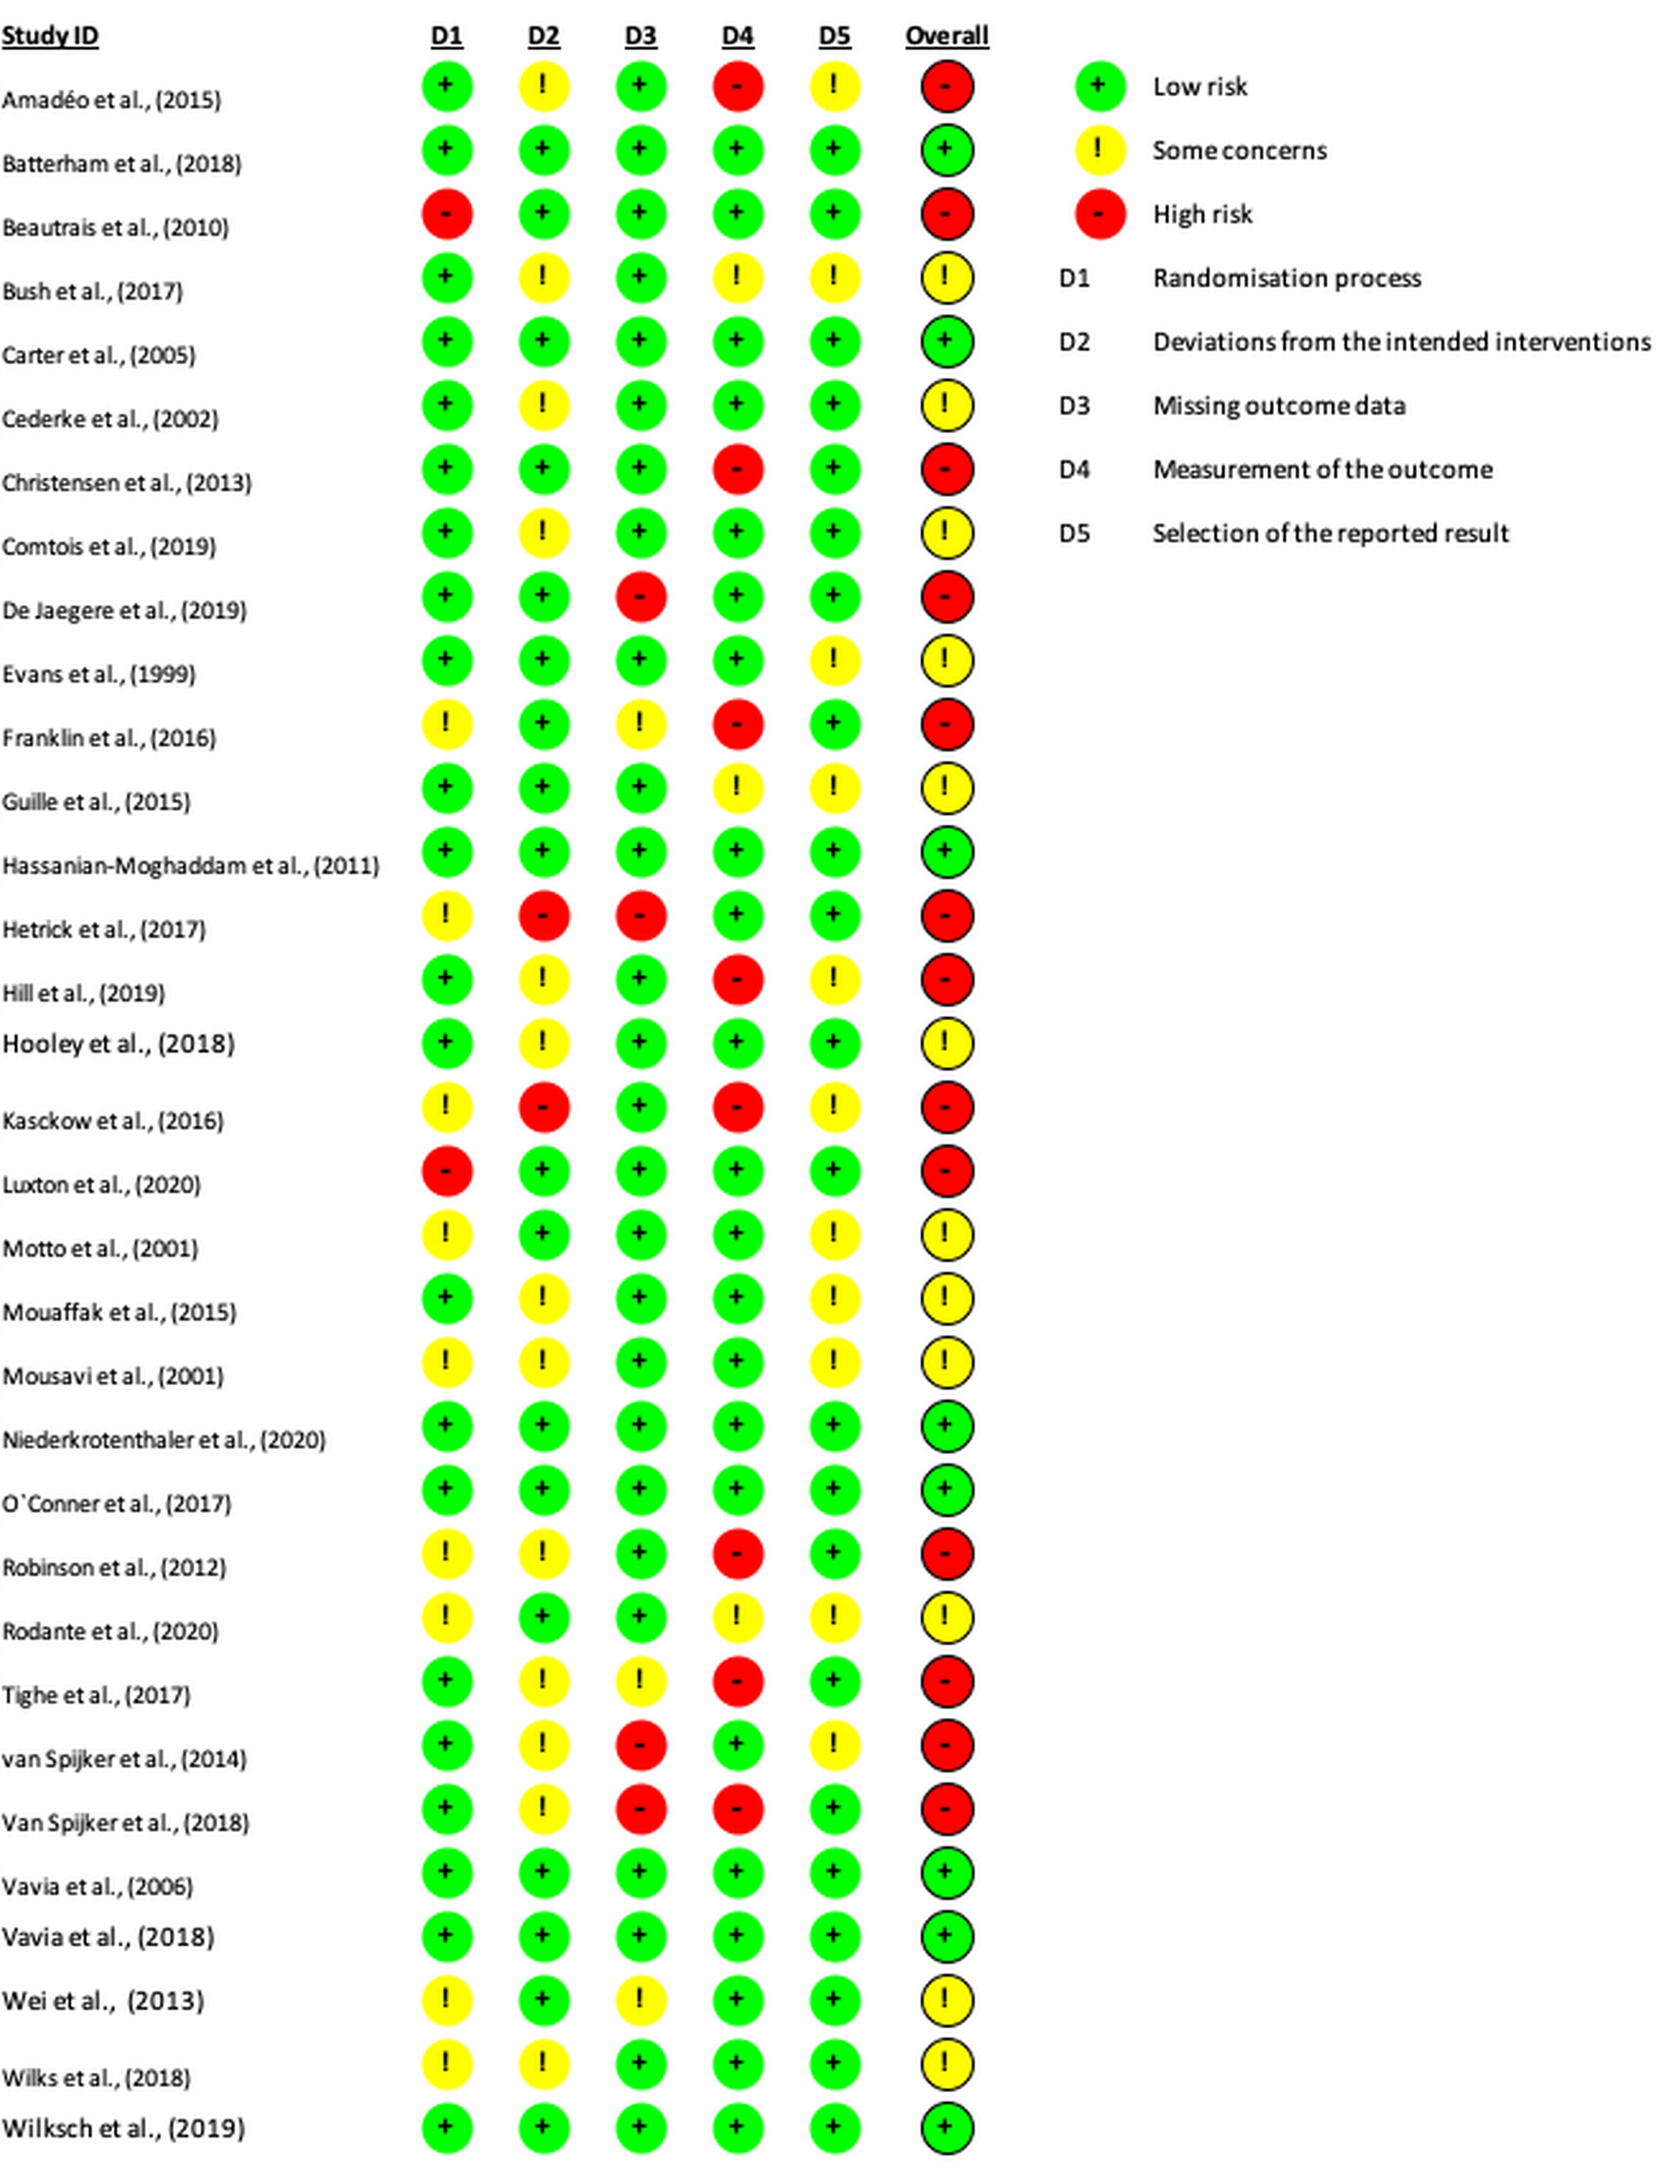
\includegraphics[width=21cm,height=\textheight]{01_Plots_Tables/RoB-II.png}
\caption{Quality Assessment of all independent studies}
\end{figure}

\hypertarget{discussion}{%
\section{Discussion}\label{discussion}}

In this meta-analysis, we examined the effectiveness of DBIs in reducing suicidal thoughts and behaviour. The quality of evidence was good, with a substantial number of~high and medium quality studies and no observed publication bias. On average, DBI reduced both suicidal thoughts and suicidal behaviour.

\hypertarget{contextualising-results-with-other-meta-analyses}{%
\subsubsection{Contextualising results with other Meta-Analyses}\label{contextualising-results-with-other-meta-analyses}}

We contextualise our findings using meta-analyses of psychotherapeutic face-to-face interventions for suicidal ideation and/or behaviour. While it can be argued that such a comparison is biased, as each meta-analysis has different inclusion criteria, designs and underlying assumptions, it nevertheless offers a rough estimation, which is important to observe which effect sizes can be expected from a suicide intervention. To maximise comparability we only include meta-analyses on psychotherapeutic face-to-face interventions, which included only RCT studies, using TAU, waitlist or attention-placebo control groups and were published in the last decade years.

We searched Web of Science using the search term: `\,``suic*'' AND ``therap*'' AND (meta-analys* OR meta analys*).' Nine meta-analyses were found (Bahji et al., 2021; Briggs et al., 2019; Chen, Cheng, Zhao, \& Zhang, 2021; Hawton et al., 2016; Hetrick, Robinson, Spittal, \& Carter, 2016; Kothgassner, Robinson, Goreis, Ougrin, \& Plener, 2020; Ougrin, Tranah, Stahl, Moran, \& Asarnow, 2015; Panos, Jackson, Hasan, \& Panos, 2014; Yuan, Kwok, \& Ougrin, 2019). One (Hetrick, Robinson, Spittal, \& Carter, 2016) did not exclude particular populations or therapeutic approaches.

\hypertarget{effectiveness-of-distance-based-interventions-dbi-for-suicidal-behaviours}{%
\paragraph{Effectiveness of Distance Based Interventions (DBI) for suicidal behaviours}\label{effectiveness-of-distance-based-interventions-dbi-for-suicidal-behaviours}}

We showed that DBI significantly reduced suicidal behaviours (\emph{SMD}= -0.06 CI95\%{[}-0.09; -0.03{]}). When comparing the results of our meta-analysis on DBI with the results of nine meta-analyses on face-to-face interventions, we found three meta-analyses with significantly higher results, while six meta-analyses reported non-significant differences. Two of the three meta-analyses reporting significantly higher results than what we found for DBI were comprised of adolescent samples (Bahji et al., 2021; Kothgassner, Robinson, Goreis, Ougrin, \& Plener, 2020); these meta-analysis used `self harm' as an outcome and showed signifcantly higher reductions by Dialectical Behavioural Therapy (DBT) at post-treatment (Bahji et al., 2021; Kothgassner, Robinson, Goreis, Ougrin, \& Plener, 2020), although their results were not significant after three months follow up (Bahji et al., 2021). In addition, one of these meta-analyses reported significantly stronger results in favour of eclectic therapy (ET) than what we found for DBI; however ET led to a significant increase in `self-harm' at three months follow-up (Bahji et al., 2021). The third meta-analysis which reported stronger results, in comparison to our results for DBI, included only psychoanalytic approaches (Briggs et al., 2019) and used suicide attempts and `self-harm' as outcomes. Psychoanalytic approaches reduced `self-harm' significantly at 6 months follow-up, although their effects were non-significant at 12 months follow-up. All of these meta-analyses predominantly used TAU as control groups.

This comparison shows that some face-to-face interventions are most likely more effective than DBI, while others are not and a few can even be harmful (Bahji et al., 2021). Furthermore, this comparison shows that research on therapeutic interventions is still too underpowered to be distinguished with statistical certainty, which emphasises the need for more research into the most promising interventions.

For such research, confidence intervals are important, as they can tell us the clinical potential of an intervention. For example, the effect size of Briggs et al. (2019) against suicide attempt episodes at 12 months follow-up is reported as Number Needed to Treat (NNT) = 7.4 CI95\% {[}Infinite; 3.6{]}. This means that while this intervention could be ineffective (infinite number of patients needed to treat), it may potentially help one in four patients, even after 12 months follow-up. In contrast, DBI reported as NNT = 29.5 CI95\% {[}59; 19.7{]}, meaning that suicidal behaviours will be reduced with a 95\% certainty, but at best one in twenty patients may be helped.

Therefore, despite small but consistent effects of DBI in comparison to face-to-face interventions DBI might be considered an option for those unable or unwilling to receive face-to-face treatment.

\hypertarget{effectiveness-of-distance-based-interventions-for-suicidal-thoughts}{%
\paragraph{Effectiveness of Distance Based Interventions for suicidal thoughts}\label{effectiveness-of-distance-based-interventions-for-suicidal-thoughts}}

According to our results suicidal thoughts are significantly reduced by Distance Based Interventions (\emph{SMD} = -0.17 CI95\%{[}-0.24; -0.11{]}). In comparison to the only meta-analysis examining face-to-face interventions and not differentiating between therapeutic approaches or populations (adults, adolescents, diagnosis), face-to-face interventions were more effective against suicidal thoughts than DBI (Hetrick, Robinson, Spittal, \& Carter, 2016). However some meta-analyses focusing on different therapeutic approaches (Bahji et al., 2021; Chen, Cheng, Zhao, \& Zhang, 2021; Kothgassner, Robinson, Goreis, Ougrin, \& Plener, 2020) also included non significantly higher results than DBI. Although we assume that this non significance was the result of lower power in comparison to Hetrick, Robinson, Spittal, and Carter (2016).

In sum we advocate a role for DBI in prevention suicidal thoughts, because of their superior scalability and promising effectiveness, given that 138 million people face suicidal ideation each year (Borges et al., 2010). It is possible that DBI have a preventive potential of between 8.6 and 18.6 million for suicidal thoughts, given an NNT = 10.45 CI95\%{[} 7.4; 16.1{]}.

\hypertarget{research-recommendations}{%
\subsubsection{Research recommendations}\label{research-recommendations}}

According to our results, aDBI (SMD= -0.14 CI95\%{[}-0.20; -0.08{]}), were as effective as hDBI (SMD= -0.08 CI95\%{[}-0.13; -0.02{]}). As aDBI promise superior scalability (Batterham et al., 2015), in contrast to hDBI, it is easier for these interventions to be implemented in studies that utilize large sample sizes, as well as replication studies.

Studies with large sample sizes or replications studies being needed, to investigate which components of DBI are most effective and which of our assumptions about how aDBI should be designed actually hold.

As it remains unclear which DBI components are most effective, or how a DBI should be designed to achieve best results. Similarly assumptions about Distance Based Interventions (DBI) for mental health lack evidence (Musiat, Goldstone, \& Tarrier, 2014), such as the superiorirtity of 24-hour availability. In contrast the best evidence derived from meta-analytical studies support the cost-effectiveness, acceptability and satisfaction of DBI by users. Notably, these evidence relates to mental health interventions in general (Eze, Mateus, \& Cravo Oliveira Hashiguchi, 2020; Musiat, Goldstone, \& Tarrier, 2014) and needs to be validated for DBI's with a suicide focus.

In this sense, the development and scientific validation of aDBIs for suicide intervention is still in its infancy and needs to addressed in future with rigour.

\hypertarget{implications-for-clinical-practice}{%
\subsubsection{Implications for clinical practice}\label{implications-for-clinical-practice}}

As mentioned Distance Based Interventions are supported by our evidence and might play a role among different levels of suicide care. Jobes, Gregorian, and Colborn (2018) in their stepped care model for suicide care denominate 5 levels of intervention, ranging from least restrictive Telephone (level 1), Brief interventions (2), outpatient care (3), partial hospitalisation (4) to most restrictive interventions like inpatient care/full hospitalisation (5). Given our evidence, we see a role of supplementation on the lower spectrum of the stepped care model, namely (human based) `telephone interventions and follow-ups' and `Brief interventions and follow-ups.'

In line with to other meta-analysis our results show that interventions are more effective in suicidal thoughts than for suicidal behaviours. This adds to the argument to provide help as early as possible, preferably to individuals with suicidal thoughts, rather than later when suicide behaviours have emerged (Jobes \& Joiner, 2019). Although they still might be helpful at this later stage, according to our result.

Further, as the density of mental health service provider is geographically unevenly distributed (Kapusta et al., 2010; Pirkola, Sund, Sailas, \& Wahlbeck, 2009) and especially as in the face of the ongoing CoV-SARS-2 pandemic caused lockdowns the barriers of face-to-face therapies are even higher and could be compensated by DBIs. Moreover, the reality of psychiatric treatment includes high costs for the individual or the health insurance (Wittchen et al., 2011), depending on insurance coverage, as well as long waiting times for patients (Zepf, Mengele, \& Hartmann, 2003). In both cases, DBI's can be an intermediate solution that bridge waiting times and thus reduces costs and human suffering. Finally, low cost aDBI's can help to expand mental health services, especially in low- and middle-income countries (LMICs), as called for by Chisholm et al. (2007) and by such contribute to the sustainable development goals for mental health set by the United Nations (Patel et al., 2018).

\hypertarget{limitations}{%
\subsection{Limitations}\label{limitations}}

Given our comprehensive approach, some potential limitations should be noted.

Firstly, it could be seen as a limitation that most studies included in this meta-analysis are already covered by previously published meta-analyses (Milner, Carter, Pirkis, Robinson, \& Spittal, 2015; Torok et al., 2020). However, these previously published meta-analyses used a methodological approach (Hedges-Olkin meta-analysis) with which only one data point per independent data-set can be included; in contrast the method used by us allows for the inclusion of all relevant data (Cheung, 2019).

Utilizing all relevant data has multiple advantages, foremost higher precision and less bias risk. (a) Including of all relevant data from a single study increases precision. Further it allows important moderator analyses to be implemented in one model, meaning evidence is weighted according to its informational value. In contrast, previous meta-analyses often had to use independent subgroup analyses, which have lower precision and only allow for indirect comparisons. (b) Bias risk, selecting one outcome per independent analysis can introduce a selection bias, as it works under the assumption that the chosen outcome is representative of all other outcomes. Based on these points and the fact that we updated and broaden the systematic searches of previous meta-analyses, the current meta-analysis substantially adds to the research field.

Despite the above stated advantages of the chosen method, this method also introduces two potential limitations. First, the employed method requires more studies to reach adequate power, risking underpowered results (Tanner-Smith \& Tipton, 2014). But our results were trustworthy, based on Profile Likelihood Plots (Raue et al., 2009) and adequately powered, according to the degrees of freedom reported by the RVE Correction (Pustejovsky \& Tipton, 2016). Second, RVE corrected models did not report heterogeneity estimations, therefore heterogeneity estimations of the Multi-level model were reported. \emph{Q-} test results are not biased by dependency and therefore statistically valid and of adequate power (Maeda \& Harwell, 2016).

\hypertarget{conclusion}{%
\subsection{Conclusion}\label{conclusion}}

The presented results are based on 35 published peer-reviewed independent RCT trials on Distance Based Interventions. With adequate power, no indication for publication bias and manageable heterogeneity, the results suggest that DBI, particularly autonomous Distance Based Interventions, are an effective possibility to support treatment, specifically in individuals with suicidal thoughts and in situations where availability of face-to-face treatments is limited. These results are encouraging as lower treatment barriers can be used to decrease treatment barriers, in turn promising a significant reduction of human suffering and health care costs.

\hypertarget{references}{%
\section{References}\label{references}}

\begingroup
\setlength{\parindent}{-0.5in}
\setlength{\leftskip}{0.5in}

References marked with an asterisk indicate studies included in the meta-analysis.

\hypertarget{refs}{}
\begin{CSLReferences}{1}{0}
\leavevmode\hypertarget{ref-amadeo2015}{}%
* Amadeo, S., Rereao, M., Malogne, A., Favro, P., Nguyen, N. L., Jehel, L., \ldots{} De Leo, D. (2015). Testing brief intervention and phone contact among subjects with suicidal behavior: {A} randomized controlled trial in {French Polynesia} in the frames of the {World Health Organization}/{Suicide Trends} in {At-Risk Territories} study. \emph{Mental Illness}, \emph{7}(2), 48--53. \url{https://doi.org/10.4081/mi.2015.5818}

\leavevmode\hypertarget{ref-americanpsychiatricassociation2013a}{}%
American Psychiatric Association. (2013). \emph{Diagnostic and {Statistical Manual} of {Mental Disorders}: {Dsm-5}}. {Amer Psychiatric Pub Incorporated}. Retrieved from \url{https://books.google.de/books?id=EIbMlwEACAAJ}

\leavevmode\hypertarget{ref-bahji2021a}{}%
Bahji, A., Pierce, M., Wong, J., Roberge, J. N., Ortega, I., \& Patten, S. (2021). Comparative {Efficacy} and {Acceptability} of {Psychotherapies} for {Self-harm} and {Suicidal Behavior Among Children} and {Adolescents}: {A Systematic Review} and {Network Meta-analysis}. \emph{JAMA Network Open}, \emph{4}(4), e216614. \url{https://doi.org/10.1001/jamanetworkopen.2021.6614}

\leavevmode\hypertarget{ref-batterham2018}{}%
* Batterham, P. J., Calear, A. L., Farrer, L., McCallum, S. M., \& Cheng, V. W. S. (2018). {FitMindKit} : {Randomised} controlled trial of an automatically tailored online program for mood, anxiety, substance use and suicidality. \emph{Internet Interventions}, \emph{12}, 91--99. \url{https://doi.org/10.1016/j.invent.2017.08.002}

\leavevmode\hypertarget{ref-batterham2015}{}%
Batterham, P. J., Ftanou, M., Pirkis, J., Brewer, J. L., Mackinnon, A. J., Beautrais, A., \ldots{} Christensen, H. (2015). A systematic review and evaluation of measures for suicidal ideation and behaviors in population-based research. \emph{Psychological Assessment}, \emph{27}(2), 501--512. \url{https://doi.org/10.1037/pas0000053}

\leavevmode\hypertarget{ref-beautrais2010}{}%
* Beautrais, A. L., Gibb, S. J., Faulkner, A., Fergusson, D. M., \& Mulder, R. T. (2010). Postcard intervention for repeat self-harm: {Randomised} controlled trial. \emph{British Journal of Psychiatry}, \emph{197}(1), 55--60. \url{https://doi.org/10.1192/bjp.bp.109.075754}

\leavevmode\hypertarget{ref-bertolote2010}{}%
* Bertolote, J. M., Fleischmann, A., De Leo, D., Phillips, M. R., Botega, N. J., Vijayakumar, L., \ldots{} Wasserman, D. (2010). Repetition of {Suicide Attempts}: {Data} from {Emergency Care Settings} in {Five Culturally Different Low-} and {Middle-Income Countries Participating} in the {WHO SUPRE-MISS Study}. \emph{Crisis-the Journal of Crisis Intervention and Suicide Prevention}, \emph{31}(4), 194--201. \url{https://doi.org/10.1027/0027-5910/a000052}

\leavevmode\hypertarget{ref-borges2010}{}%
Borges, G., Nock, M. K., Haro Abad, J. M., Hwang, I., Sampson, N. A., Alonso, J., \ldots{} Kessler, R. C. (2010). Twelve-{Month Prevalence} of and {Risk Factors} for {Suicide Attempts} in the {World Health Organization World Mental Health Surveys}. \emph{Journal of Clinical Psychiatry}, \emph{71}(12), 1617--1628. \url{https://doi.org/10.4088/JCP.08m04967blu}

\leavevmode\hypertarget{ref-briggs2019}{}%
Briggs, S., Netuveli, G., Gould, N., Gkaravella, A., Gluckman, N. S., Kangogyere, P., \ldots{} Lindner, R. (2019). The effectiveness of {Psychoanalytic}/{Psychodynamic} psychotherapy for reducing suicide attempts and self-harm: {Systematic} review and meta-analysis. \emph{The British Journal of Psychiatry : The Journal of Mental Science}, \emph{214}(06), 320--328. \url{https://doi.org/10.1192/bjp.2019.33}

\leavevmode\hypertarget{ref-bruffaerts2011}{}%
Bruffaerts, R., Demyttenaere, K., Hwang, I., Chiu, W.-T., Sampson, N., Kessler, R. C., \ldots{} Nock, M. K. (2011). Treatment of suicidal people around the world. \emph{The British Journal of Psychiatry}, \emph{199}(1), 64--70. \url{https://doi.org/10.1192/bjp.bp.110.084129}

\leavevmode\hypertarget{ref-bush2017}{}%
* Bush, N. E., Smolenski, D. J., Denneson, L. M., Williams, H. B., Thomas, E. K., \& Dobscha, S. K. (2017). A {Virtual Hope Box}: {Randomized Controlled Trial} of a {Smartphone App} for {Emotional Regulation} and {Coping With Distress}. \emph{Psychiatric Services}, \emph{68}(4), 330--336. \url{https://doi.org/10.1176/appi.ps.201600283}

\leavevmode\hypertarget{ref-carter2007}{}%
* Carter, Gregory L., Clover, K., Whyte, I. M., Dawson, A. H., \& D'Este, C. (2007). Postcards from the {EDge}: 24-{Month} outcomes of a randomised controlled trial for hospital-treated self-poisoning. \emph{British Journal of Psychiatry}, \emph{191}, 548--553. \url{https://doi.org/10.1192/bjp.bp.107.038406}

\leavevmode\hypertarget{ref-carter2013}{}%
* Carter, Gregory L., Clover, K., Whyte, I. M., Dawson, A. H., \& D'Este, C. (2013). Postcards from the {EDge}: 5-{Year} outcomes of a randomised controlled trial for hospital-treated self-poisoning. \emph{British Journal of Psychiatry}, \emph{202}(5), 372--380. \url{https://doi.org/10.1192/bjp.bp.112.112664}

\leavevmode\hypertarget{ref-carter2005}{}%
* Carter, Gregory L., Clover, K., Whyte, I. M., Dawson, A. H., \& Este, C. D. (2005). Postcards from the {EDge} project: {Randomised} controlled trial of an intervention using postcards to reduce repetition of hospital treated deliberate self poisoning. \emph{BMJ (Clinical Research Ed.)}, \emph{331}(7520), 805. \url{https://doi.org/10.1136/bmj.38579.455266.E0}

\leavevmode\hypertarget{ref-cedereke2002}{}%
* Cedereke, M., Monti, K., \& Ojehagen, A. (2002). Telephone contact with patients in the year after a suicide attempt: {Does} it affect treatment attendance and outcome? {A} randomised controlled study. \emph{European Psychiatry}, \emph{17}(2), 82--91. \url{https://doi.org/10.1016/S0924-9338(02)00632-6}

\leavevmode\hypertarget{ref-chen2021}{}%
Chen, S., Cheng, Y., Zhao, W., \& Zhang, Y. (2021). Effects of dialectical behaviour therapy on reducing self‐harming behaviours and negative emotions in patients with borderline personality disorder: {A} meta‐analysis. \emph{Journal of Psychiatric and Mental Health Nursing}, \emph{28}(6), 1128--1139. \url{https://doi.org/10.1111/jpm.12797}

\leavevmode\hypertarget{ref-cheung2019}{}%
Cheung, M. W.-L. (2019). A {Guide} to {Conducting} a {Meta-Analysis} with {Non-Independent Effect Sizes}. \emph{Neuropsychology Review}, \emph{29}(4), 387--396. \url{https://doi.org/10.1007/s11065-019-09415-6}

\leavevmode\hypertarget{ref-chisholm2007}{}%
Chisholm, D., Flisher, A. J., Lund, C., Patel, V., Saxena, S., Thornicroft, G., \& Tomlinson, M. (2007). Scale up services for mental disorders: {A} call for action. \emph{Lancet (London, England)}, \emph{370}(9594), 1241--1252. \url{https://doi.org/10.1016/S0140-6736(07)61242-2}

\leavevmode\hypertarget{ref-christensen2013}{}%
* Christensen, H., Farrer, L., Batterham, P. J., Mackinnon, A., Griffiths, K. M., \& Donker, T. (2013). The effect of a web-based depression intervention on suicide ideation: {Secondary} outcome from a randomised controlled trial in a helpline. \emph{Bmj Open}, \emph{3}(6), e002886. \url{https://doi.org/10.1136/bmjopen-2013-002886}

\leavevmode\hypertarget{ref-comtois2019}{}%
* Comtois, K. A., Kerbrat, A. H., DeCou, C. R., Atkins, D. C., Majeres, J. J., Baker, J. C., \& Ries, R. K. (2019). Effect of {Augmenting Standard Care} for {Military Personnel With Brief Caring Text Messages} for {Suicide Prevention A Randomized Clinical Trial}. \emph{Jama Psychiatry}, \emph{76}(5), 474--483. \url{https://doi.org/10.1001/jamapsychiatry.2018.4530}

\leavevmode\hypertarget{ref-dejaegere2019}{}%
* De Jaegere, E., van Landschoot, R., van Heeringen, K., van Spijker, B. A. J., Kerkhof, A. J. F. M., Mokkenstorm, J. K., \& Portzky, G. (2019). The online treatment of suicidal ideation: {A} randomised controlled trial of an unguided web-based intervention. \emph{Behaviour Research and Therapy}, \emph{119}, 103406. \url{https://doi.org/10.1016/j.brat.2019.05.003}

\leavevmode\hypertarget{ref-evans1999}{}%
* Evans, M. O., Morgan, H. G., Hayward, A., \& Gunnell, D. J. (1999). Crisis telephone consultation for deliberate self-harm patients: {Effects} on repetition. \emph{British Journal of Psychiatry}, \emph{175}, 23--27. \url{https://doi.org/10.1192/bjp.175.1.23}

\leavevmode\hypertarget{ref-eze2020}{}%
Eze, N. D., Mateus, C., \& Cravo Oliveira Hashiguchi, T. (2020). Telemedicine in the {OECD}: {An} umbrella review of clinical and cost-effectiveness, patient experience and implementation. \emph{PLOS ONE}, \emph{15}(8), e0237585. \url{https://doi.org/10.1371/journal.pone.0237585}

\leavevmode\hypertarget{ref-fernandez2021}{}%
Fernandez, E., Woldgabreal, Y., Day, A., Pham, T., Gleich, B., \& Aboujaoude, E. (2021). Live psychotherapy by video versus {In}‐person: {A Meta}‐analysis of efficacy and its relationship to types and targets of treatment. \emph{Clinical Psychology \& Psychotherapy}, cpp.2594. \url{https://doi.org/10.1002/cpp.2594}

\leavevmode\hypertarget{ref-fernandez-castilla2021}{}%
Fernández-Castilla, B., Declercq, L., Jamshidi, L., Beretvas, S. N., Onghena, P., \& Van den Noortgate, W. (2021). Detecting {Selection Bias} in {Meta-Analyses} with {Multiple Outcomes}: {A Simulation Study}. \emph{The Journal of Experimental Education}, \emph{89}(1), 125--144. \url{https://doi.org/10.1080/00220973.2019.1582470}

\leavevmode\hypertarget{ref-franklin2016}{}%
* Franklin, J. C., Fox, K. R., Franklin, C. R., Kleiman, E. M., Ribeiro, J. D., Jaroszewski, A. C., \ldots{} Nock, M. K. (2016). A brief mobile app reduces nonsuicidal and suicidal self-injury: {Evidence} from three randomized controlled trials. \emph{Journal of Consulting and Clinical Psychology}, \emph{84}(6), 544--557. \url{https://doi.org/10.1037/ccp0000093}

\leavevmode\hypertarget{ref-guille2015}{}%
* Guille, C., Zhao, Z., Krystal, J., Nichols, B., Brady, K., \& Sen, S. (2015). Web-{Based Cognitive Behavioral Therapy Intervention} for the {Prevention} of {Suicidal Ideation} in {Medical Interns}: {A Randomized Clinical Trial}. \emph{JAMA Psychiatry}, \emph{72}(12), 1192. \url{https://doi.org/10.1001/jamapsychiatry.2015.1880}

\leavevmode\hypertarget{ref-hassanian-moghaddam2011}{}%
* Hassanian-Moghaddam, H., Sarjami, S., Kolahi, A.-A., \& Carter, G. L. (2011). Postcards in {Persia}: {Randomised} controlled trial to reduce suicidal behaviours 12 months after hospital-treated self-poisoning. \emph{British Journal of Psychiatry}, \emph{198}(4), 309--316. \url{https://doi.org/10.1192/bjp.bp.109.067199}

\leavevmode\hypertarget{ref-hassanian-moghaddam2017}{}%
* Hassanian-Moghaddam, H., Sarjami, S., Kolahi, A.-A., Lewin, T., \& Carter, G. (2017). Postcards in {Persia}: {A Twelve} to {Twenty-Four Month Follow-up} of a {Randomized Controlled Trial} for {Hospital-Treated Deliberate Self-Poisoning}. \emph{Archives of Suicide Research}, \emph{21}(1), 138--154. \url{https://doi.org/10.1080/13811118.2015.1004473}

\leavevmode\hypertarget{ref-hawton2016}{}%
Hawton, K., Witt, K. G., Salisbury, T. L. T., Arensman, E., Gunnell, D., Hazell, P., \ldots{} van Heeringen, K. (2016). Psychosocial interventions following self-harm in adults: A systematic review and meta-analysis. \emph{The Lancet Psychiatry}, \emph{3}(8), 740--750. \url{https://doi.org/10.1016/S2215-0366(16)30070-0}

\leavevmode\hypertarget{ref-hedges2010}{}%
Hedges, L. V., Tipton, E., \& Johnson, M. C. (2010). Robust variance estimation in meta-regression with dependent effect size estimates. \emph{Research Synthesis Methods}, \emph{1}(1), 39--65. \url{https://doi.org/10.1002/jrsm.5}

\leavevmode\hypertarget{ref-hetrick2016}{}%
Hetrick, S. E., Robinson, J., Spittal, M. J., \& Carter, G. (2016). Effective psychological and psychosocial approaches to reduce repetition of self-harm: A systematic review, meta-analysis and meta-regression. \emph{BMJ Open}, \emph{6}(9), e011024. \url{https://doi.org/10.1136/bmjopen-2016-011024}

\leavevmode\hypertarget{ref-hetrick2017}{}%
* Hetrick, S. E., Yuen, H. P., Bailey, E., Cox, G. R., Templer, K., Rice, S. M., \ldots{} Robinson, J. (2017). Internet-based cognitive behavioural therapy for young people with suicide-related behaviour ({Reframe-IT}): {A} randomised controlled trial. \emph{Evidence-Based Mental Health}, \emph{20}(3), 76--82. \url{https://doi.org/10.1136/eb-2017-102719}

\leavevmode\hypertarget{ref-hill2019}{}%
* Hill, R. M., \& Pettit, J. W. (2019). Pilot randomized controlled trial of {LEAP}: {A} selective preventive intervention to reduce adolescents' perceived burdensomeness. \emph{JOURNAL OF CLINICAL CHILD AND ADOLESCENT PSYCHOLOGY}, \emph{48}, S45--S56. \url{https://doi.org/10.1080/15374416.2016.1188705}

\leavevmode\hypertarget{ref-hooley2018}{}%
* Hooley, J. M., Fox, K. R., Wang, S. B., \& Kwashie, A. N. D. (2018). Novel online daily diary interventions for nonsuicidal self-injury: {A} randomized controlled trial. \emph{BMC Psychiatry}, \emph{18}(1). \url{https://doi.org/10.1186/s12888-018-1840-6}

\leavevmode\hypertarget{ref-jobes2018}{}%
Jobes, D. A., Gregorian, M. J., \& Colborn, V. A. (2018). A stepped care approach to clinical suicide prevention. \emph{Psychological Services}, \emph{15}(3), 243--250. \url{https://doi.org/10.1037/ser0000229}

\leavevmode\hypertarget{ref-jobes2019}{}%
Jobes, D. A., \& Joiner, T. E. (2019). Reflections on {Suicidal Ideation}. \emph{Crisis-the Journal of Crisis Intervention and Suicide Prevention}, \emph{40}(4), 227--230. \url{https://doi.org/10.1027/0227-5910/a000615}

\leavevmode\hypertarget{ref-joiner2005}{}%
Joiner, T. (2005). \emph{Why people die by suicide.} {Cambridge, MA, US}: {Harvard University Press}.

\leavevmode\hypertarget{ref-kapusta2010}{}%
Kapusta, N. D., Posch, M., Niederkrotenthaler, T., Fischer-Kern, M., Etzersdorfer, E., \& Sonneck, G. (2010). Availability of {Mental Health Service Providers} and {Suicide Rates} in {Austria}: {A Nationwide Study}, \emph{61}(12), 6.

\leavevmode\hypertarget{ref-kasckow2016}{}%
* Kasckow, J., Zickmund, S., Gurklis, J., Luther, J., Fox, L., Taylor, M., \ldots{} Haas, G. L. (2016). Using telehealth to augment an intensive case monitoring program in veterans with schizophrenia and suicidal ideation: {A} pilot trial, 14.

\leavevmode\hypertarget{ref-kothgassner2020a}{}%
Kothgassner, O. D., Robinson, K., Goreis, A., Ougrin, D., \& Plener, P. L. (2020). Does treatment method matter? {A} meta-analysis of the past 20 years of research on therapeutic interventions for self-harm and suicidal ideation in adolescents. \emph{Borderline Personality Disorder and Emotion Dysregulation}, \emph{7}(1), 9. \url{https://doi.org/10.1186/s40479-020-00123-9}

\leavevmode\hypertarget{ref-luxton2020}{}%
* Luxton, D. D., Smolenski, D. J., Reger, M. A., Relova, R. M. V., \& Skopp, N. A. (2020). Caring {E}‐mails for {Military} and {Veteran Suicide Prevention}: {A Randomized Controlled Trial}. \emph{Suicide and Life-Threatening Behavior}, \emph{50}(1), 300--314. \url{https://doi.org/10.1111/sltb.12589}

\leavevmode\hypertarget{ref-maeda2016}{}%
Maeda, Y., \& Harwell, M. R. (2016). Guidelines for {Using} the {Q Test} in {Meta-Analysis}, \emph{28}(1), 18.

\leavevmode\hypertarget{ref-milner2015}{}%
Milner, A. J., Carter, G., Pirkis, J., Robinson, J., \& Spittal, M. J. (2015). Letters, green cards, telephone calls and postcards: {Systematic} and meta-analytic review of brief contact interventions for reducing self-harm, suicide attempts and suicide. \emph{British Journal of Psychiatry}, \emph{206}(3), 184--190. \url{https://doi.org/10.1192/bjp.bp.114.147819}

\leavevmode\hypertarget{ref-moeyaert2017}{}%
Moeyaert, M., Ugille, M., Natasha Beretvas, S., Ferron, J., Bunuan, R., \& Van den Noortgate, W. (2017). Methods for dealing with multiple outcomes in meta-analysis: {A} comparison between averaging effect sizes, robust variance estimation and multilevel meta-analysis. \emph{Null}, \emph{20}(6), 559--572. \url{https://doi.org/10.1080/13645579.2016.1252189}

\leavevmode\hypertarget{ref-motto2001}{}%
* Motto, J. A., \& Bostrom, A. G. (2001). A {Randomized Controlled Trial} of {Postcrisis Suicide Prevention}. \emph{Psychiatric Services}, \emph{52}(6), 828--833. \url{https://doi.org/10.1176/appi.ps.52.6.828}

\leavevmode\hypertarget{ref-mouaffak2015}{}%
* Mouaffak, F., Marchand, A., Castaigne, E., Arnoux, A., \& Hardy, P. (2015). {OSTA} program: {A French} follow up intervention program for suicide prevention. \emph{Psychiatry Research}, \emph{230}(3), 913--918. \url{https://doi.org/10.1016/j.psychres.2015.11.024}

\leavevmode\hypertarget{ref-mousavi2014}{}%
* Mousavi, S. G., Zohreh, R., Maracy, M. R., Ebrahimi, A., \& Sharbafchi, M. R. (2014). The efficacy of telephonic follow up in prevention of suicidal reattempt in patients with suicide attempt history. \emph{Advanced Biomedical Research}, 6.

\leavevmode\hypertarget{ref-musiat2014}{}%
Musiat, P., Goldstone, P., \& Tarrier, N. (2014). Understanding the acceptability of e-mental health - attitudes and expectations towards computerised self-help treatments for mental health problems. \emph{BMC Psychiatry}, \emph{14}(1), 109. \url{https://doi.org/10.1186/1471-244X-14-109}

\leavevmode\hypertarget{ref-niederkrotenthaler2020}{}%
* Niederkrotenthaler, T., \& Till, B. (2020). Effects of suicide awareness materials on individuals with recent suicidal ideation or attempt: {Online} randomised controlled trial. \emph{British Journal of Psychiatry}, \emph{217}(6), 693--700. \url{https://doi.org/10.1192/bjp.2019.259}

\leavevmode\hypertarget{ref-oconnor2017}{}%
* O'Connor, R. C., Ferguson, E., Scott, F., Smyth, R., McDaid, D., Park, A.-L., \ldots{} Armitage, C. J. (2017). A brief psychological intervention to reduce repetition of self-harm in patients admitted to hospital following a suicide attempt: {A} randomised controlled trial. \emph{The Lancet. Psychiatry}, \emph{4}(6), 451--460. \url{https://doi.org/10.1016/S2215-0366(17)30129-3}

\leavevmode\hypertarget{ref-ougrin2015}{}%
Ougrin, D., Tranah, T., Stahl, D., Moran, P., \& Asarnow, J. R. (2015). Therapeutic {Interventions} for {Suicide Attempts} and {Self-Harm} in {Adolescents}: {Systematic Review} and {Meta-Analysis}. \emph{Journal of the American Academy of Child \& Adolescent Psychiatry}, \emph{54}(2), 97--107.e2. \url{https://doi.org/10.1016/j.jaac.2014.10.009}

\leavevmode\hypertarget{ref-page2021}{}%
Page, M. J., McKenzie, J. E., Bossuyt, P. M., Boutron, I., Hoffmann, T. C., Mulrow, C. D., \ldots{} Moher, D. (2021). The {PRISMA} 2020 statement: {An} updated guideline for reporting systematic reviews. \emph{BMJ (Clinical Research Ed.)}, n71. \url{https://doi.org/10.1136/bmj.n71}

\leavevmode\hypertarget{ref-panos2014}{}%
Panos, P. T., Jackson, J. W., Hasan, O., \& Panos, A. (2014). Meta-{Analysis} and {Systematic Review Assessing} the {Efficacy} of {Dialectical Behavior Therapy} ({DBT}). \emph{Research on Social Work Practice}, \emph{24}(2), 213--223. \url{https://doi.org/10.1177/1049731513503047}

\leavevmode\hypertarget{ref-park2019}{}%
Park, S., \& Beretvas, S. N. (2019). Synthesizing effects for multiple outcomes per study using robust variance estimation versus the three-level model. \emph{Behav Res}, \emph{51}(1), 152--171. \url{https://doi.org/10.3758/s13428-018-1156-y}

\leavevmode\hypertarget{ref-patel2018}{}%
Patel, V., Saxena, S., Lund, C., Thornicroft, G., Baingana, F., Bolton, P., \ldots{} UnÜtzer, Jü. (2018). The {Lancet Commission} on global mental health and sustainable development. \emph{The Lancet}, \emph{392}(10157), 1553--1598. \url{https://doi.org/10.1016/S0140-6736(18)31612-X}

\leavevmode\hypertarget{ref-pirkola2009}{}%
Pirkola, S., Sund, R., Sailas, E., \& Wahlbeck, K. (2009). Community mental-health services and suicide rate in {Finland}: A nationwide small-area analysis. \emph{The Lancet}, \emph{373}(9658), 147--153. \url{https://doi.org/10.1016/S0140-6736(08)61848-6}

\leavevmode\hypertarget{ref-pustejovsky2021a}{}%
Pustejovsky, J. E. (2021). \emph{{clubSandwich}: {Cluster-robust} (sandwich) variance estimators with small-sample corrections}. manual. Retrieved from \url{https://CRAN.R-project.org/package=clubSandwich}

\leavevmode\hypertarget{ref-pustejovsky2016}{}%
Pustejovsky, J. E., \& Tipton, E. (2016). Small sample methods for cluster-robust variance estimation and hypothesis testing in fixed effects models. Retrieved from \url{http://arxiv.org/abs/1601.01981}

\leavevmode\hypertarget{ref-pustejovsky2021}{}%
Pustejovsky, J. E., \& Tipton, E. (2021). Meta-analysis with {Robust Variance Estimation}: {Expanding} the {Range} of {Working Models}. \emph{Prevention Science}. \url{https://doi.org/10.1007/s11121-021-01246-3}

\leavevmode\hypertarget{ref-rcoreteam2020}{}%
R Core Team. (2020). \emph{R: {A} language and environment for statistical computing}. manual, {Vienna, Austria}. Retrieved from \url{https://www.R-project.org/}

\leavevmode\hypertarget{ref-raue2009}{}%
Raue, A., Kreutz, C., Maiwald, T., Bachmann, J., Schilling, M., Klingmüller, U., \& Timmer, J. (2009). Structural and practical identifiability analysis of partially observed dynamical models by exploiting the profile likelihood. \emph{Bioinformatics}, \emph{25}(15), 1923--1929. \url{https://doi.org/10.1093/bioinformatics/btp358}

\leavevmode\hypertarget{ref-renkewitz2019}{}%
Renkewitz, F., \& Keiner, M. (2019). How to {Detect Publication Bias} in {Psychological Research}: {A Comparative Evaluation} of {Six Statistical Methods}. \emph{Zeitschrift für Psychologie}, \emph{227}(4), 261--279. \url{https://doi.org/10.1027/2151-2604/a000386}

\leavevmode\hypertarget{ref-robinson2012}{}%
* Robinson, J., Yuen, H. P., Gook, S., Hughes, A., Cosgrave, E., Killackey, E., \ldots{} Yung, A. (2012). Can receipt of a regular postcard reduce suicide-related behaviour in young help seekers? {A} randomized controlled trial: {A} postcard study for at-{Risk} young help seekers. \emph{Early Intervention in Psychiatry}, \emph{6}(2), 145--152. \url{https://doi.org/10.1111/j.1751-7893.2011.00334.x}

\leavevmode\hypertarget{ref-rodante2020}{}%
* Rodante, D. E., Kaplan, M. I., Olivera Fedi, R., Gagliesi, P., Pascali, A., José Quintero, P. S., \ldots{} Daray, F. M. (2020). {CALMA}, a {Mobile Health Application}, as an {Accessory} to {Therapy} for {Reduction} of {Suicidal} and {Non-Suicidal Self-Injured Behaviors}: {A Pilot Cluster Randomized Controlled Trial}. \emph{Null}, 1--18. \url{https://doi.org/10.1080/13811118.2020.1834476}

\leavevmode\hypertarget{ref-sterne2019}{}%
Sterne, J. A. C., Savović, J., Page, M. J., Elbers, R. G., Blencowe, N. S., Boutron, I., \ldots{} Higgins, J. P. T. (2019). {RoB} 2: {A} revised tool for assessing risk of bias in randomised trials. \emph{BMJ (Clinical Research Ed.)}, l4898. \url{https://doi.org/10.1136/bmj.l4898}

\leavevmode\hypertarget{ref-tanner-smith2014}{}%
Tanner-Smith, E. E., \& Tipton, E. (2014). Robust variance estimation with dependent effect sizes: {Practical} considerations including a software tutorial in {Stata} and {\textsc{Spss}}: {Robust} variance estimation, \emph{5}(1), 13--30. \url{https://doi.org/10.1002/jrsm.1091}

\leavevmode\hypertarget{ref-tighe2017}{}%
* Tighe, J., Shand, F., Ridani, R., Mackinnon, A., De La Mata, N., \& Christensen, H. (2017). Ibobbly mobile health intervention for suicide prevention in {Australian Indigenous} youth: {A} pilot randomised controlled trial. \emph{BMJ Open}, \emph{7}(1), e013518. \url{https://doi.org/10.1136/bmjopen-2016-013518}

\leavevmode\hypertarget{ref-torok2020}{}%
Torok, M., Han, J., Baker, S., Werner-Seidler, A., Wong, I., Larsen, M. E., \& Christensen, H. (2020). Suicide prevention using self-guided digital interventions: {A} systematic review and meta-analysis of randomised controlled trials. \emph{The Lancet Digital Health}, \emph{2}(1), e25--e36. \url{https://doi.org/10.1016/S2589-7500(19)30199-2}

\leavevmode\hypertarget{ref-vaiva2018}{}%
* Vaiva, G., Berrouiguet, S., Walter, M., Courtet, P., Ducrocq, F., Jardon, V., \ldots{} Goldstein, P. (2018). Combining {Postcards}, {Crisis Cards}, and {Telephone Contact Into} a {Decision-Making Algorithm} to {Reduce Suicide Reattempt}: {A Randomized Clinical Trial} of a {Personalized Brief Contact Intervention}. \emph{The Journal of Clinical Psychiatry}, \emph{79}(6). \url{https://doi.org/10.4088/JCP.17m11631}

\leavevmode\hypertarget{ref-vaiva2006}{}%
* Vaiva, G., Vaiva, G., Ducrocq, F., Meyer, P., Mathieu, D., Philippe, A., \ldots{} Goudemand, M. (2006). Effect of telephone contact on further suicide attempts in patients discharged from an emergency department: {Randomised} controlled study. \emph{BMJ (Clinical Research Ed.)}, \emph{332}(7552), 1241--1245. \url{https://doi.org/10.1136/bmj.332.7552.1241}

\leavevmode\hypertarget{ref-vandennoortgate2013}{}%
Van den Noortgate, W., López-López, J. A., Marín-Martínez, F., \& Sánchez-Meca, J. (2013). Three-level meta-analysis of dependent effect sizes. \emph{Behavior Research Methods}, \emph{45}(2), 576--594. \url{https://doi.org/10.3758/s13428-012-0261-6}

\leavevmode\hypertarget{ref-vandennoortgate2015}{}%
Van den Noortgate, W., López-López, J. A., Marín-Martínez, F., \& Sánchez-Meca, J. (2015). Meta-analysis of multiple outcomes: {A} multilevel approach. \emph{Behavior Research Methods}, \emph{47}(4), 1274--1294. \url{https://doi.org/10.3758/s13428-014-0527-2}

\leavevmode\hypertarget{ref-vanspijker2014}{}%
* van Spijker, B. A. J., van Straten, A., \& Kerkhof, A. J. F. M. (2014). Effectiveness of {Online Self-Help} for {Suicidal Thoughts}: {Results} of a {Randomised Controlled Trial}. \emph{PLoS ONE}, \emph{9}(2), e90118. \url{https://doi.org/10.1371/journal.pone.0090118}

\leavevmode\hypertarget{ref-vanspijker2018}{}%
* van Spijker, B. A., Werner-Seidler, A., Batterham, P. J., Mackinnon, A., Calear, A. L., Gosling, J. A., \ldots{} Christensen, H. (2018). Effectiveness of a {Web-Based Self-Help Program} for {Suicidal Thinking} in an {Australian Community Sample}: {Randomized Controlled Trial}. \emph{Journal of Medical Internet Research}, \emph{20}(2), e15. \url{https://doi.org/10.2196/jmir.8595}

\leavevmode\hypertarget{ref-viechtbauer2010c}{}%
Viechtbauer, W. (2010). Conducting {Meta-Analyses} in {R} with the metafor {Package}. \emph{Journal of Statistical Software}, \emph{36}(3). \url{https://doi.org/10.18637/jss.v036.i03}

\leavevmode\hypertarget{ref-wei2013}{}%
* Wei, S., Liu, L., Bi, B., Li, H., Hou, J., Tan, S., \ldots{} Liu, Y. (2013). An {Intervention} and {Follow-Up Study Following} a {Suicide Attempt} in the {Emergency Departments} of {Four General Hospitals} in {Shenyang}, {China}. \emph{Crisis-the Journal of Crisis Intervention and Suicide Prevention}, \emph{34}(2), 107--115. \url{https://doi.org/10.1027/0227-5910/a000181}

\leavevmode\hypertarget{ref-wilks2018}{}%
* Wilks, C. R., Lungu, A., Ang, S. Y., Matsumiya, B., Yin, Q., \& Linehan, M. M. (2018). A randomized controlled trial of an {Internet} delivered dialectical behavior therapy skills training for suicidal and heavy episodic drinkers. \emph{Journal of Affective Disorders}, \emph{232}, 219--228. \url{https://doi.org/10.1016/j.jad.2018.02.053}

\leavevmode\hypertarget{ref-wittchen2011a}{}%
Wittchen, H. U., Jacobi, F., Rehm, J., Gustavsson, A., Svensson, M., Jönsson, B., \ldots{} Steinhausen, H.-C. (2011). The size and burden of mental disorders and other disorders of the brain in {Europe} 2010. \emph{European Neuropsychopharmacology}, \emph{21}(9), 655--679. \url{https://doi.org/10.1016/j.euroneuro.2011.07.018}

\leavevmode\hypertarget{ref-worldhealthorganization2021}{}%
World Health Organization. (2021). \emph{Suicide worldwide in 2019: {Global} health estimates}. {Geneva}: {World Health Organization}. Retrieved from \url{https://apps.who.int/iris/handle/10665/341728}

\leavevmode\hypertarget{ref-yuan2019}{}%
Yuan, S. N. V., Kwok, K. H. R., \& Ougrin, D. (2019). Treatment {Engagement} in {Specific Psychological Treatment} vs. {Treatment} as {Usual} for {Adolescents With Self-Harm}: {Systematic Review} and {Meta-Analysis}. \emph{Frontiers in Psychology}, \emph{10}, 104. \url{https://doi.org/10.3389/fpsyg.2019.00104}

\leavevmode\hypertarget{ref-zepf2003}{}%
Zepf, S., Mengele, U., \& Hartmann, S. (2003). Zum Stand der ambulanten psychotherapeutischen Versorgung der Erwachsenen in der Bundesrepublik Deutschland. \emph{Psychotherapie, Psychosomatik, medizinische Psychologie}, \emph{53}(3/4), 152--162. \url{https://doi.org/10.1055/s-2003-38004}

\leavevmode\hypertarget{ref-zuromski2019}{}%
Zuromski, K. L., Bernecker, S. L., Gutierrez, P. M., Joiner, T. E., King, A. J., Liu, H., \ldots{} Kessler, R. C. (2019). Assessment of a {Risk Index} for {Suicide Attempts Among US Army Soldiers With Suicide Ideation}: {Analysis} of {Data From} the {Army Study} to {Assess Risk} and {Resilience} in {Servicemembers} ({Army STARRS}). \emph{JAMA Network Open}, \emph{2}(3), e190766. \url{https://doi.org/10.1001/jamanetworkopen.2019.0766}

\end{CSLReferences}

\endgroup


\end{document}
